%% LyX 2.3.6.1 created this file.  For more info, see http://www.lyx.org/.
%% Do not edit unless you really know what you are doing.
\documentclass[oneside,english]{amsart}
\usepackage[T1]{fontenc}
\usepackage[latin9]{inputenc}
\usepackage{babel}
\usepackage{mathtools}
\usepackage{amstext}
\usepackage{amsthm}
\usepackage{graphicx}
\usepackage[unicode=true,pdfusetitle,
 bookmarks=true,bookmarksnumbered=false,bookmarksopen=false,
 breaklinks=false,pdfborder={0 0 1},backref=false,colorlinks=false]
 {hyperref}

\makeatletter
%%%%%%%%%%%%%%%%%%%%%%%%%%%%%% Textclass specific LaTeX commands.
\numberwithin{equation}{section}
\numberwithin{figure}{section}
\numberwithin{table}{section}

\makeatother

\begin{document}
\title{On the correctness of implementing random permutation as sorting random
keys}
\author{Xiang Gao}
\begin{abstract}
This documentation studies how many bits are required in random keys
in order to implement random permutation of $N$ numbers. Fewer bits
means faster radix sort but poorer randomness. This documentation
shows that, in order to generate a random permutaion of $N$ numbers
with correctness probability $\ge q$, the random numbers are required
to have at least $\left\lceil \log_{2}\left(N-\frac{6N^{2}+1}{12\cdot\log q}\right)\right\rceil $
bits.
\end{abstract}

\maketitle

\section{Introduction}

A common way to implement random permutation of $N$ numbers on GPU
is by generating $N$ random numbers as keys then sorting. This implementation
is correct only when these $N$ random numbers are different, because
stable sort algorithms will not permute two identical keys, making
$\left(0,1\right)$ more preferred than $\left(1,0\right)$. If these
random keys had infinite precision, then duplicate keys was not a
problem, because the probability of this case was $0$. However, for
finite precision random numbers, this is not the case.

Though facing correctness issue, for better performance, these $N$
random numbers are usually generated independently and there is no
effort to guarantee they are different with each other. We want to
study the probability of getting duplicate keys. From this probability,
we can know how many bits are required in random keys in order to
get a good enough randomness.

\section{The probability of getting non-duplicate keys}

An $m$ bit random number has $M=2^{m}$ different values. Getting
$N$ independent random numbers from an $m$ bit random generator
is equivalent to drawing $N$ samples from a size $M$ pool with replacement,
with uniform distribution, and order matters. Therefore, there are
in total $M^{N}$ different cases. Within these cases, $P(M,N)$ of
them don't have duplicate samples, where the $P\left(M,N\right)$
is often written as $n\mathrm{P}r$, is defined by 
\[
P\left(M,N\right)\coloneqq\frac{M!}{\left(M-N\right)!}.
\]
So the probability of getting non-duplicating keys is
\[
\Pr\left[\text{unique samples}\right]=\frac{P\left(M,N\right)}{M^{N}}
\]

According to a narrowed version of Stirling's formula by Robbins\cite{10.2307/2308012}
\[
\sqrt{2\pi}n^{n+\frac{1}{2}}e^{-n}e^{\frac{1}{12n+1}}\leq n!\leq\sqrt{2\pi}n^{n+\frac{1}{2}}e^{-n}e^{\frac{1}{12n}}
\]
we then have
\[
\frac{M^{M+\frac{1}{2}}e^{-M}e^{\frac{1}{12M+1}}}{\left(M-N\right)^{\left(M-N\right)+\frac{1}{2}}e^{-\left(M-N\right)}e^{\frac{1}{12\left(M-N\right)}}}\leq P\left(M,N\right)\leq\frac{M^{M+\frac{1}{2}}e^{-M}e^{\frac{1}{12M}}}{\left(M-N\right)^{\left(M-N\right)+\frac{1}{2}}e^{-\left(M-N\right)}e^{\frac{1}{12\left(M-N\right)+1}}}
\]
which simplify to
\[
\frac{M^{M+\frac{1}{2}}\cdot e^{-N}}{\left(M-N\right)^{\left(M-N\right)+\frac{1}{2}}}\cdot e^{\frac{1}{12M+1}-\frac{1}{12\left(M-N\right)}}\leq P\left(M,N\right)\leq\frac{M^{M+\frac{1}{2}}\cdot e^{-N}}{\left(M-N\right)^{\left(M-N\right)+\frac{1}{2}}}\cdot e^{\frac{1}{12M}-\frac{1}{12\left(M-N\right)+1}}
\]
so
\begin{multline*}
\frac{M^{(M-N)+\frac{1}{2}}\cdot e^{-N}}{\left(M-N\right)^{\left(M-N\right)+\frac{1}{2}}}\cdot e^{\frac{1}{12M+1}-\frac{1}{12\left(M-N\right)}}\leq\\
\Pr\left[\text{unique samples}\right]\leq\frac{M^{(M-N)+\frac{1}{2}}}{\left(M-N\right)^{\left(M-N\right)+\frac{1}{2}}e^{N}}\cdot e^{\frac{1}{12M}-\frac{1}{12\left(M-N\right)+1}}
\end{multline*}
which simplify to
\begin{multline*}
\left(\frac{M}{M-N}\right)^{(M-N)+\frac{1}{2}}\cdot e^{-N}\cdot e^{\frac{1}{12M+1}-\frac{1}{12\left(M-N\right)}}\leq\\
\Pr\left[\text{unique samples}\right]\leq\left(\frac{M}{M-N}\right)^{(M-N)+\frac{1}{2}}\cdot e^{-N}\cdot e^{\frac{1}{12M}-\frac{1}{12\left(M-N\right)+1}}
\end{multline*}
Let's write the above inequality as
\[
f\left(M,N\right)\leq\Pr\left[\text{unique samples}\right]\leq g\left(M,N\right)
\]


\section{Bound}

We want to make sure the probability of getting non-duplicate samples
above a certain threshold: 
\begin{equation}
\Pr\left[\text{unique samples}\right]\geq q\label{eq:prthres}
\end{equation}
As long as $f\left(M,N\right)\geq q$, equation (\ref{eq:prthres})
will be automatically satisfied. Note that
\begin{multline*}
f\left(M,N\right)=\left(\frac{M}{M-N}\right)^{(M-N)+\frac{1}{2}}\cdot e^{-N}\cdot e^{\frac{1}{12M+1}-\frac{1}{12\left(M-N\right)}}\\
=\left(1+\frac{N}{M-N}\right)^{(M-N)+\frac{1}{2}}\cdot e^{-N}\cdot e^{\frac{1}{12M+1}-\frac{1}{12\left(M-N\right)}}
\end{multline*}
then
\[
\log f\left(M,N\right)=\left(M-N+\frac{1}{2}\right)\log\left(1+\frac{N}{M-N}\right)-N+\frac{1}{12M+1}-\frac{1}{12\left(M-N\right)}
\]
since
\[
\log\left(1+\frac{N}{M-N}\right)\geq\frac{N}{M-N}-\frac{1}{2}\left(\frac{N}{M-N}\right)^{2}
\]
\[
M-N+\frac{1}{2}\geq M-N
\]
\[
\frac{1}{12M+1}\geq0
\]
we have
\begin{multline*}
\log f\left(M,N\right)\geq\left(M-N\right)\left[\frac{N}{M-N}-\frac{1}{2}\left(\frac{N}{M-N}\right)^{2}\right]-N-\frac{1}{12\left(M-N\right)}\\
=-\frac{1}{12}\cdot\frac{6N^{2}+1}{M-N}
\end{multline*}
So, as long as
\[
-\frac{1}{12}\cdot\frac{6N^{2}+1}{M-N}\geq\log q
\]
that is
\[
M\geq N-\frac{6N^{2}+1}{12\cdot\log q}
\]
there is a guarantee that the probability of getting unique keys is
above $q$.

\newpage{}

\section{Summary}

So, in order to have $N$ different random numbers at probability
$\ge q$, you will need an
\[
m=\left\lceil \log_{2}\left(N-\frac{6N^{2}+1}{12\cdot\log q}\right)\right\rceil 
\]
bit random number generator.

Plotting the above equation for $q$= 0.9. The plot of the above function
is shown below, the $x$-axis is $\log_{2}N$, the $y$-axis is $m$

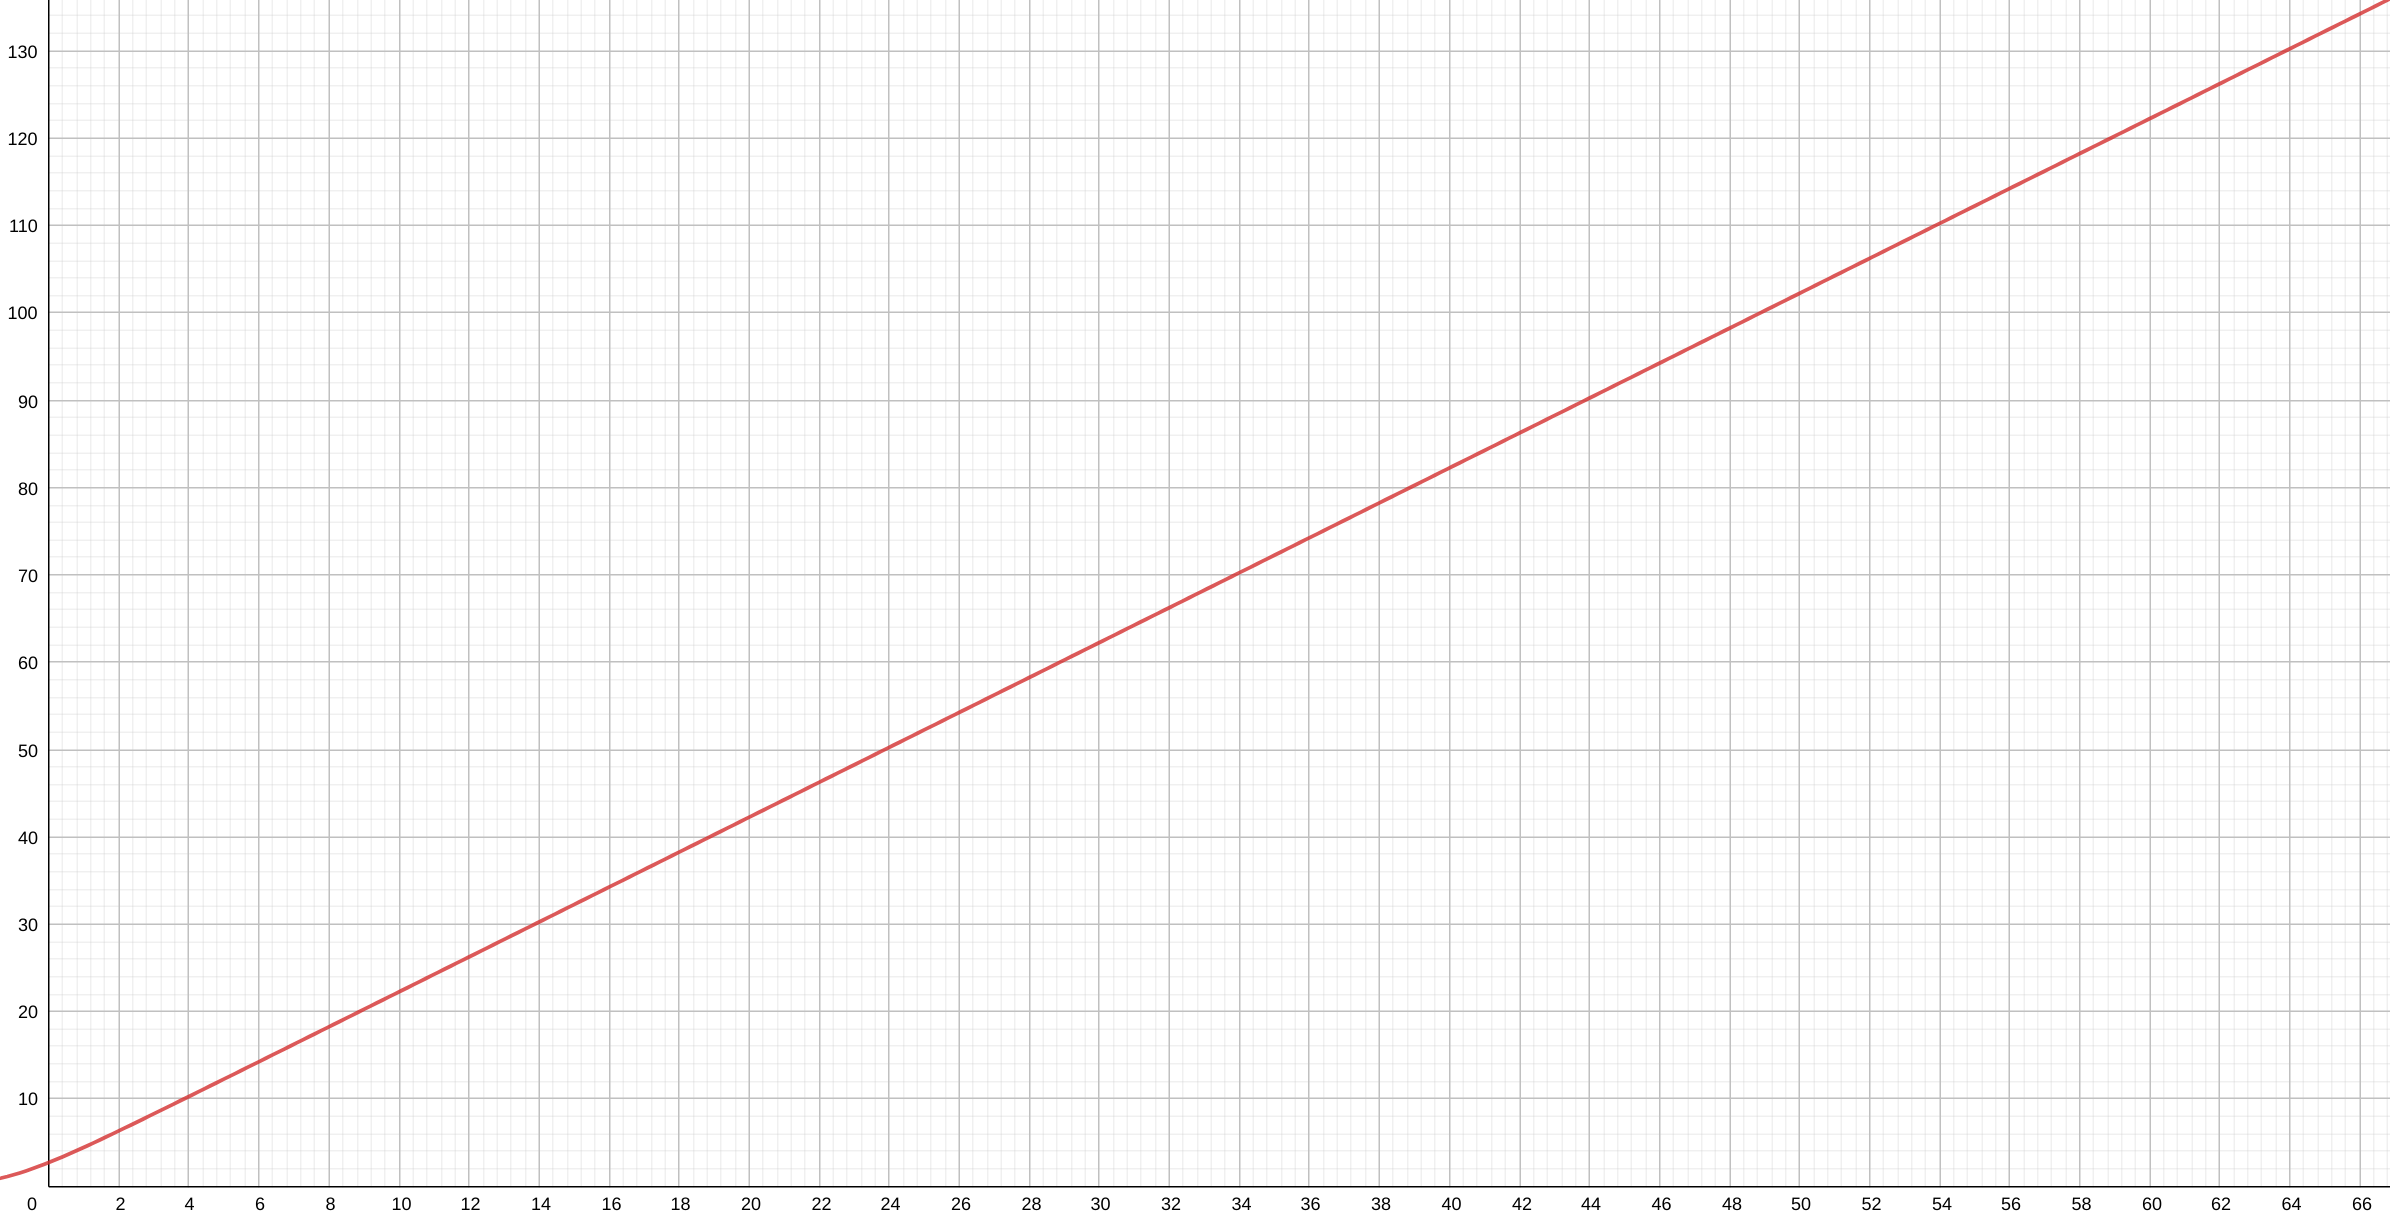
\includegraphics[width=1\linewidth]{plot}

\bibliographystyle{plain}
\bibliography{randperm}

\end{document}
